\documentclass{beamer}
\let\Tiny=\tiny % Gets rid of font warning.
\usepackage{lmodern,amsmath,amssymb,listings}
\usepackage{spot}
\usepackage{fancybox}
\usepackage[skins,listings]{tcolorbox}
\tcbset{enhanced}
\usepackage{fancyvrb}
\usepackage[latin1]{inputenc}
\usepackage[T1]{fontenc}
\usetheme{Warsaw}
\setbeamertemplate{navigation symbols}{} % turn off slide navigation buttons at the bottom
\setbeamersize{text margin left=6mm, text margin right=6mm} 

\title[Implementing WGFEM]{Implementing the Weak Galerkin F.E.M.}
\subtitle{With a Focus on Generality}

\author{Stephen Harris \\ \texttt{scharris@ualr.edu}}
\date{Nov. 7, 2013}


\begin{document}

\begin{frame}
  \titlepage
\end{frame}

\begin{frame}
  \frametitle{Outline}
  \tableofcontents[pausesections]
\end{frame}

\section{Generality Goal}
\subsection{Generality Defined}

\begin{frame}
  \frametitle{What is Meant by Generality Here?}
  \pause
  The ability to most easily solve the widest variety of problems
    \begin{align*}
      \spot<7>{\mathfrak{a}}(u_h,v) & = (\spot<4>{f},v)\quad\quad\quad \forall{v} \in \spot<6>{V_{h0}} \\
      u_h & = \spot<4>{g} \text{ on } \partial\spot<5>{\Omega}
    \end{align*}
    for solution $u_h$ in piecewise polynomial approximation space $V_h$ on mesh \spot<5>{$M_h$} of \spot<5>{$\Omega$}.
  \pause

  \begin{block}{Method Should Allow ``Mix and Match'' of Parts}
    Should allow the ``actors'' above to easily be varied independently:
    \pause
    \begin{enumerate}[<+->]
      \item functions $f$ and $g$
      \item mesh $M_h$ on which $V_h$ members are piecewise polynomial
      \item approximation space, by choice of \emph{degree constraints} on polynomial pieces of $V_h$ members -- by monomial degree or maximum variable degree
      \item bilinear form $\mathfrak{a}: V_h \times V_h \rightarrow \mathbb{R}$
    \end{enumerate}
  \end{block}

\end{frame}

\begin{frame}
  \frametitle{How General is the Implementation?}
  \pause
  \begin{itemize}[<+->]
    \item Many problems solvable without code additions or changes.
      \begin{itemize}[<+->]
        \item Allow arbitrary functions for $f$ and $g$.
        \item Provided Meshes
          \begin{itemize}
            \item Triangle meshes from mesh generator (Gmsh).
            \item Rectangle meshes for any number of space dimensions.
          \end{itemize}
        \item Basis -- Support arbitrary \emph{degree constraints} for approximating polynomials on interiors and sides separately,
          using either monomial or variable degree.
        \item Laplace bilinear form provided. 
      \end{itemize}
    \item Extensible in areas expected to frequently need changes.
      \begin{itemize}
        \item New problems solved by plugging in new code at \emph{plugin points}.
        \item Major plugin points are provided for
          \begin{itemize}
            \item variational bilinear form, $\mathfrak{a}$
            \item mesh -- Arbitrary polytope meshes for any space dimension can be supported. No uniformity requirements.
          \end{itemize}
        \item No mesh or vbf is ``built in'': provided ones use plugin system.
        \item Only \emph{new} aspects have to be coded for, thought about, and tested. Core method does not change.
      \end{itemize}
  \end{itemize}
\end{frame}

\subsection{The Means -- Abstraction and Modularity}

\subsubsection{Components: Limited Roles, Limited Knowledge}

\begin{frame}
  \frametitle{How? Components: Limited Roles, Limited Knowledge}
  Divide system into components having clear, limited roles.
  \pause
  \tcbset{left=1mm,right=1mm,bottom=1mm,top=1mm}
  \tcbox{Limited Role} \raisebox{3mm}{$\implies$} \raisebox{-0.2mm}{\tcbox{Limited Knowledge}}\\
  A component having a limited role means it also should have no knowledge of other components' internal workings.\\
  \pause
  Components should only depend on exposed operations of other components and their \emph{documented} behavior (usually the names).\\
  \pause
  Keep connections between components at a minimum!
  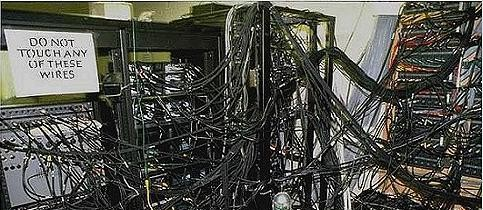
\includegraphics[height=3.5cm]{crazy-wiring.jpg}
\end{frame}

\subsubsection{Components for the WG Method}

\begin{frame}
  \frametitle{How Generality is Achieved: Abstraction and Modularity}
  Divide system into components having clear, limited roles.\\
  \pause
  \tcbset{colback =red!5!white, colframe =red!75!black, left=0mm,right=0mm,bottom=0mm,top=0mm}
  \begin{block}{Major Components}
    \tcbox{\shadowbox{Mesh}}
    \raisebox{1.4mm}{\shadowbox{WGrad Solver}}
    \raisebox{1.4mm}{\shadowbox{Basis}}
    \raisebox{1.25mm}{\shadowbox{Proj}}
    \tcbox{\shadowbox{VBF}}
    \raisebox{3.4mm}{\fbox{WG Solver}}
  \end{block}
  \pause
  \begin{block}{Auxiliary Types \& Components}
    \shadowbox{Monomial}
    \shadowbox{Polynomial}
    \shadowbox{Vector Monomial}
    \shadowbox{Weak Grad}
    \shadowbox{WG Solution}
    \raisebox{2mm}{\fbox{Error Norms}}
    \raisebox{2mm}{\fbox{Quadrature}}
    \raisebox{2mm}{\fbox{Linear Algebra}}
  \end{block}
  \pause
  \raisebox{-2mm}{\shadowbox{Shadowed}} components represent \emph{types}, with custom ops.\\
  \pause
  \raisebox{-2mm}{\tcbox{Enclosed}} types represent abstract
  types, or \emph{contracts}, as a set of operations which actual ``plugged in'' types must implement.
\end{frame}

\subsection{Bringing Components Together - Example}

\begin{frame}[fragile]{Bringing Components Together -- Example Run}
  \tcbset{colback =red!5!white, colframe =red!75!black, left=0mm,right=0mm,bottom=0mm,top=0mm, tcbox raise base}
  \begin{Verbatim}[gobble=4, commandchars=\\\{\}, fontsize=\small, fontfamily=tt]
    fn u(x: &[R]) -> R  \{ cos(x[0]) + sin(x[1]) \} \textcolor{gray}{// exact solution}
    fn f(x: &[R]) -> R  \{ cos(x[0]) + sin(x[1]) \} \textcolor{gray}{// var form rhs}
    fn g(x: &[R]) -> R  \{ u(x) \} \textcolor{gray}{                 // boundary cond}

    let \textcolor{green!50!black}{mesh} = \spot{~RectMesh}::new(~[0.,0.], ~[2*pi,2*pi], ~[500, 500]);

    let \textcolor{blue}{basis} = &WGBasis::new(\tcbox{\textcolor{green!50!black}{mesh}}, MaxMonDeg(3), MaxMonDeg(2));

    let \textcolor{orange!50!red}{vbf} = \spot{VBFLaplace}::new(None, \textcolor{blue}{basis});

    let wg_sol = wg_solver::solve(\tcbox{\textcolor{orange!50!red}{vbf}}, \textcolor{blue}{basis}, f, g);

    let err = err_L2_norm(u, &wg_sol);
  \end{Verbatim}
  \footnotesize {
    \textcolor{gray}{// \spot{\emph{Any} types satisfying the respective contracts are usable at these spots.}}\\
    \textcolor{gray}{// The types are only manipulated via contract-guaranteed operations within\\
      // the method -- black boxes with contract ops being the external controls.}
  }
\end{frame}

\section{Concepts}

\subsection{Mesh Elements}

\subsubsection{Oriented Shapes}

\begin{frame}
  \frametitle{Oriented Shapes}
  \begin{columns}
    \column{.50\textwidth}
      \frame{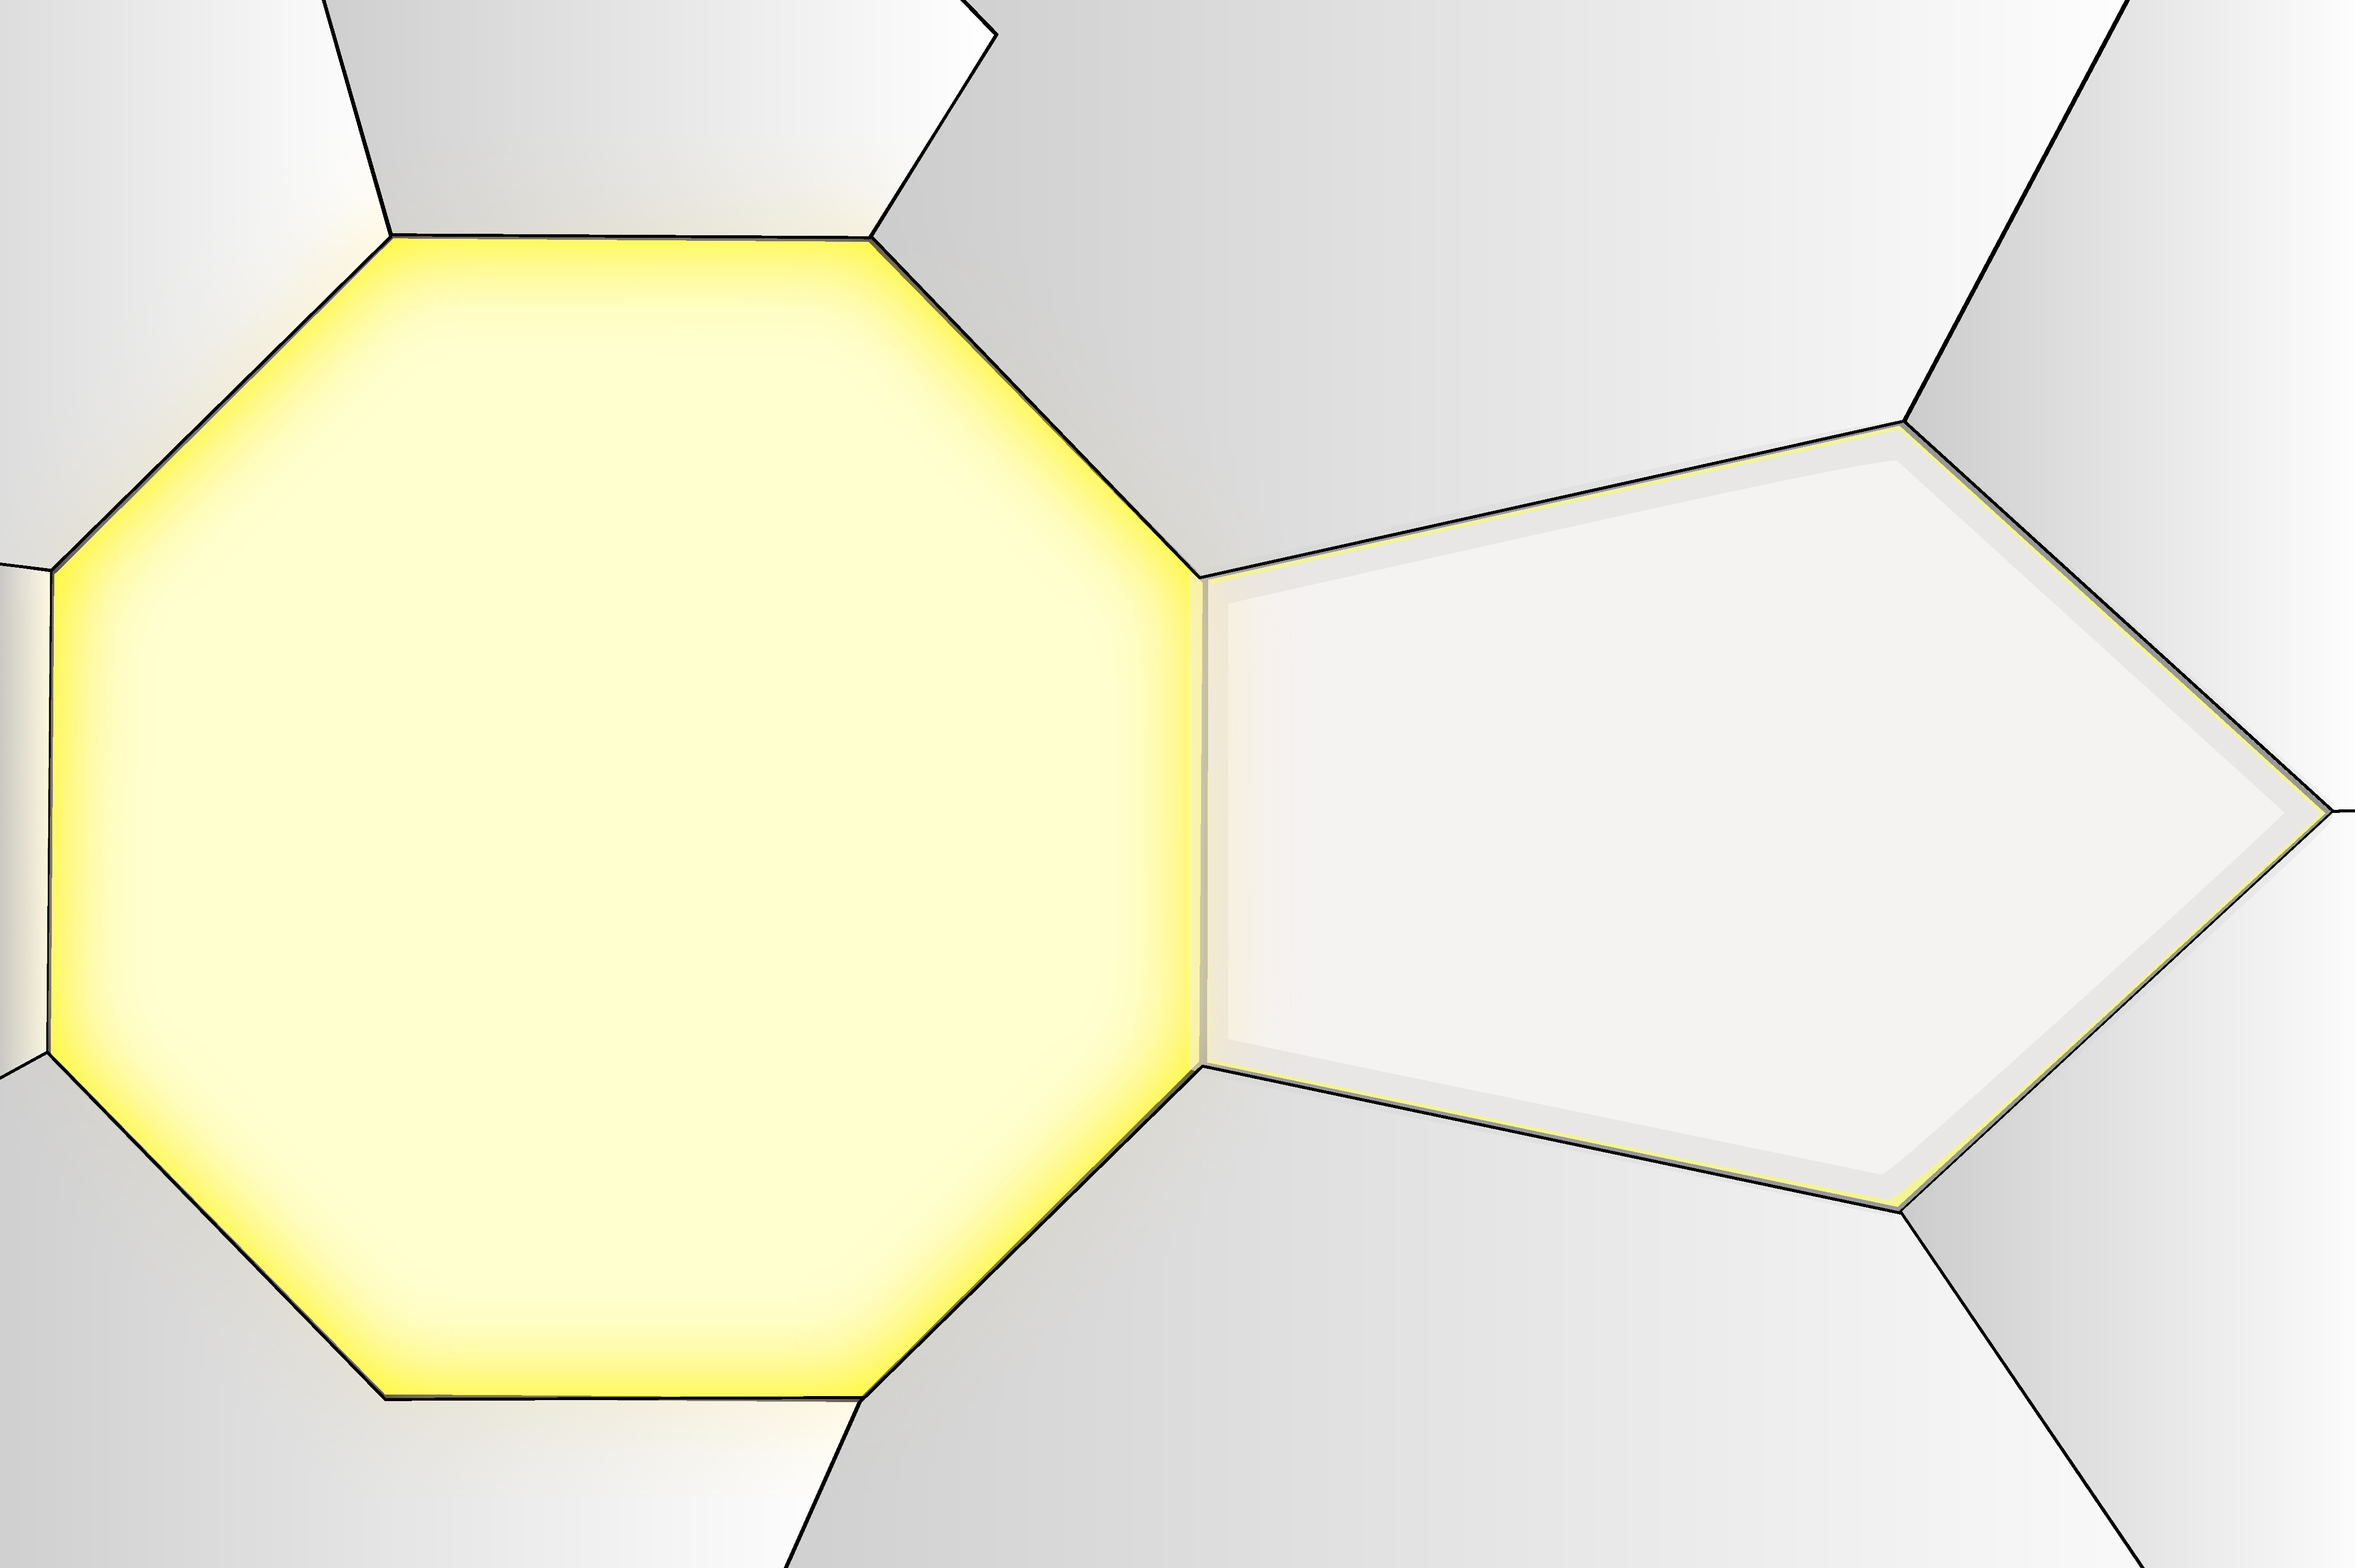
\includegraphics[width=6cm, height=4cm]{two_fes.pdf}}
    \column{.50\textwidth}
      \pause
      \begin{itemize}[<+->]
        \item Elements may have, \emph{independently} of each other, any \textbf{shape} and \textbf{orientation}.
        \item Two elements are of the same \textbf{\emph{oriented shape}} iff some translation takes one's points into and onto the other's.
      \end{itemize}
  \end{columns}
  
  \begin{itemize}[<+->]
    \item Is an abstraction of a finite element ignoring its position.
    \item Many calculations can be done on an oriented shape just once instead of individually on all finite elements of the shape.
    \item Mesh must assign an oriented shape for \emph{each} finite element. 
    \item Mesh will identify oriented shapes by enumerating them in some order of its choosing.
      Enumeration makes iteration and use as an array index easy. Mesh internally can store more information.
  \end{itemize}
\end{frame}

\subsubsection{Identifying Finite Elements and Non-Boundary Sides}

\begin{frame}
  \frametitle{Identifying Finite Elements and Non-Boundary Sides}
  \begin{columns}
    \column{.50\textwidth}
      \begin{itemize}[<+->]
        \item Mesh will need to provide identifiers for the \emph{\textbf{support faces}} for the basis shape functions.
        \item Only interiors and non-boundary sides will host shape functions.
      \end{itemize}
    \column{.50\textwidth}
      \alt<-2> {\frame{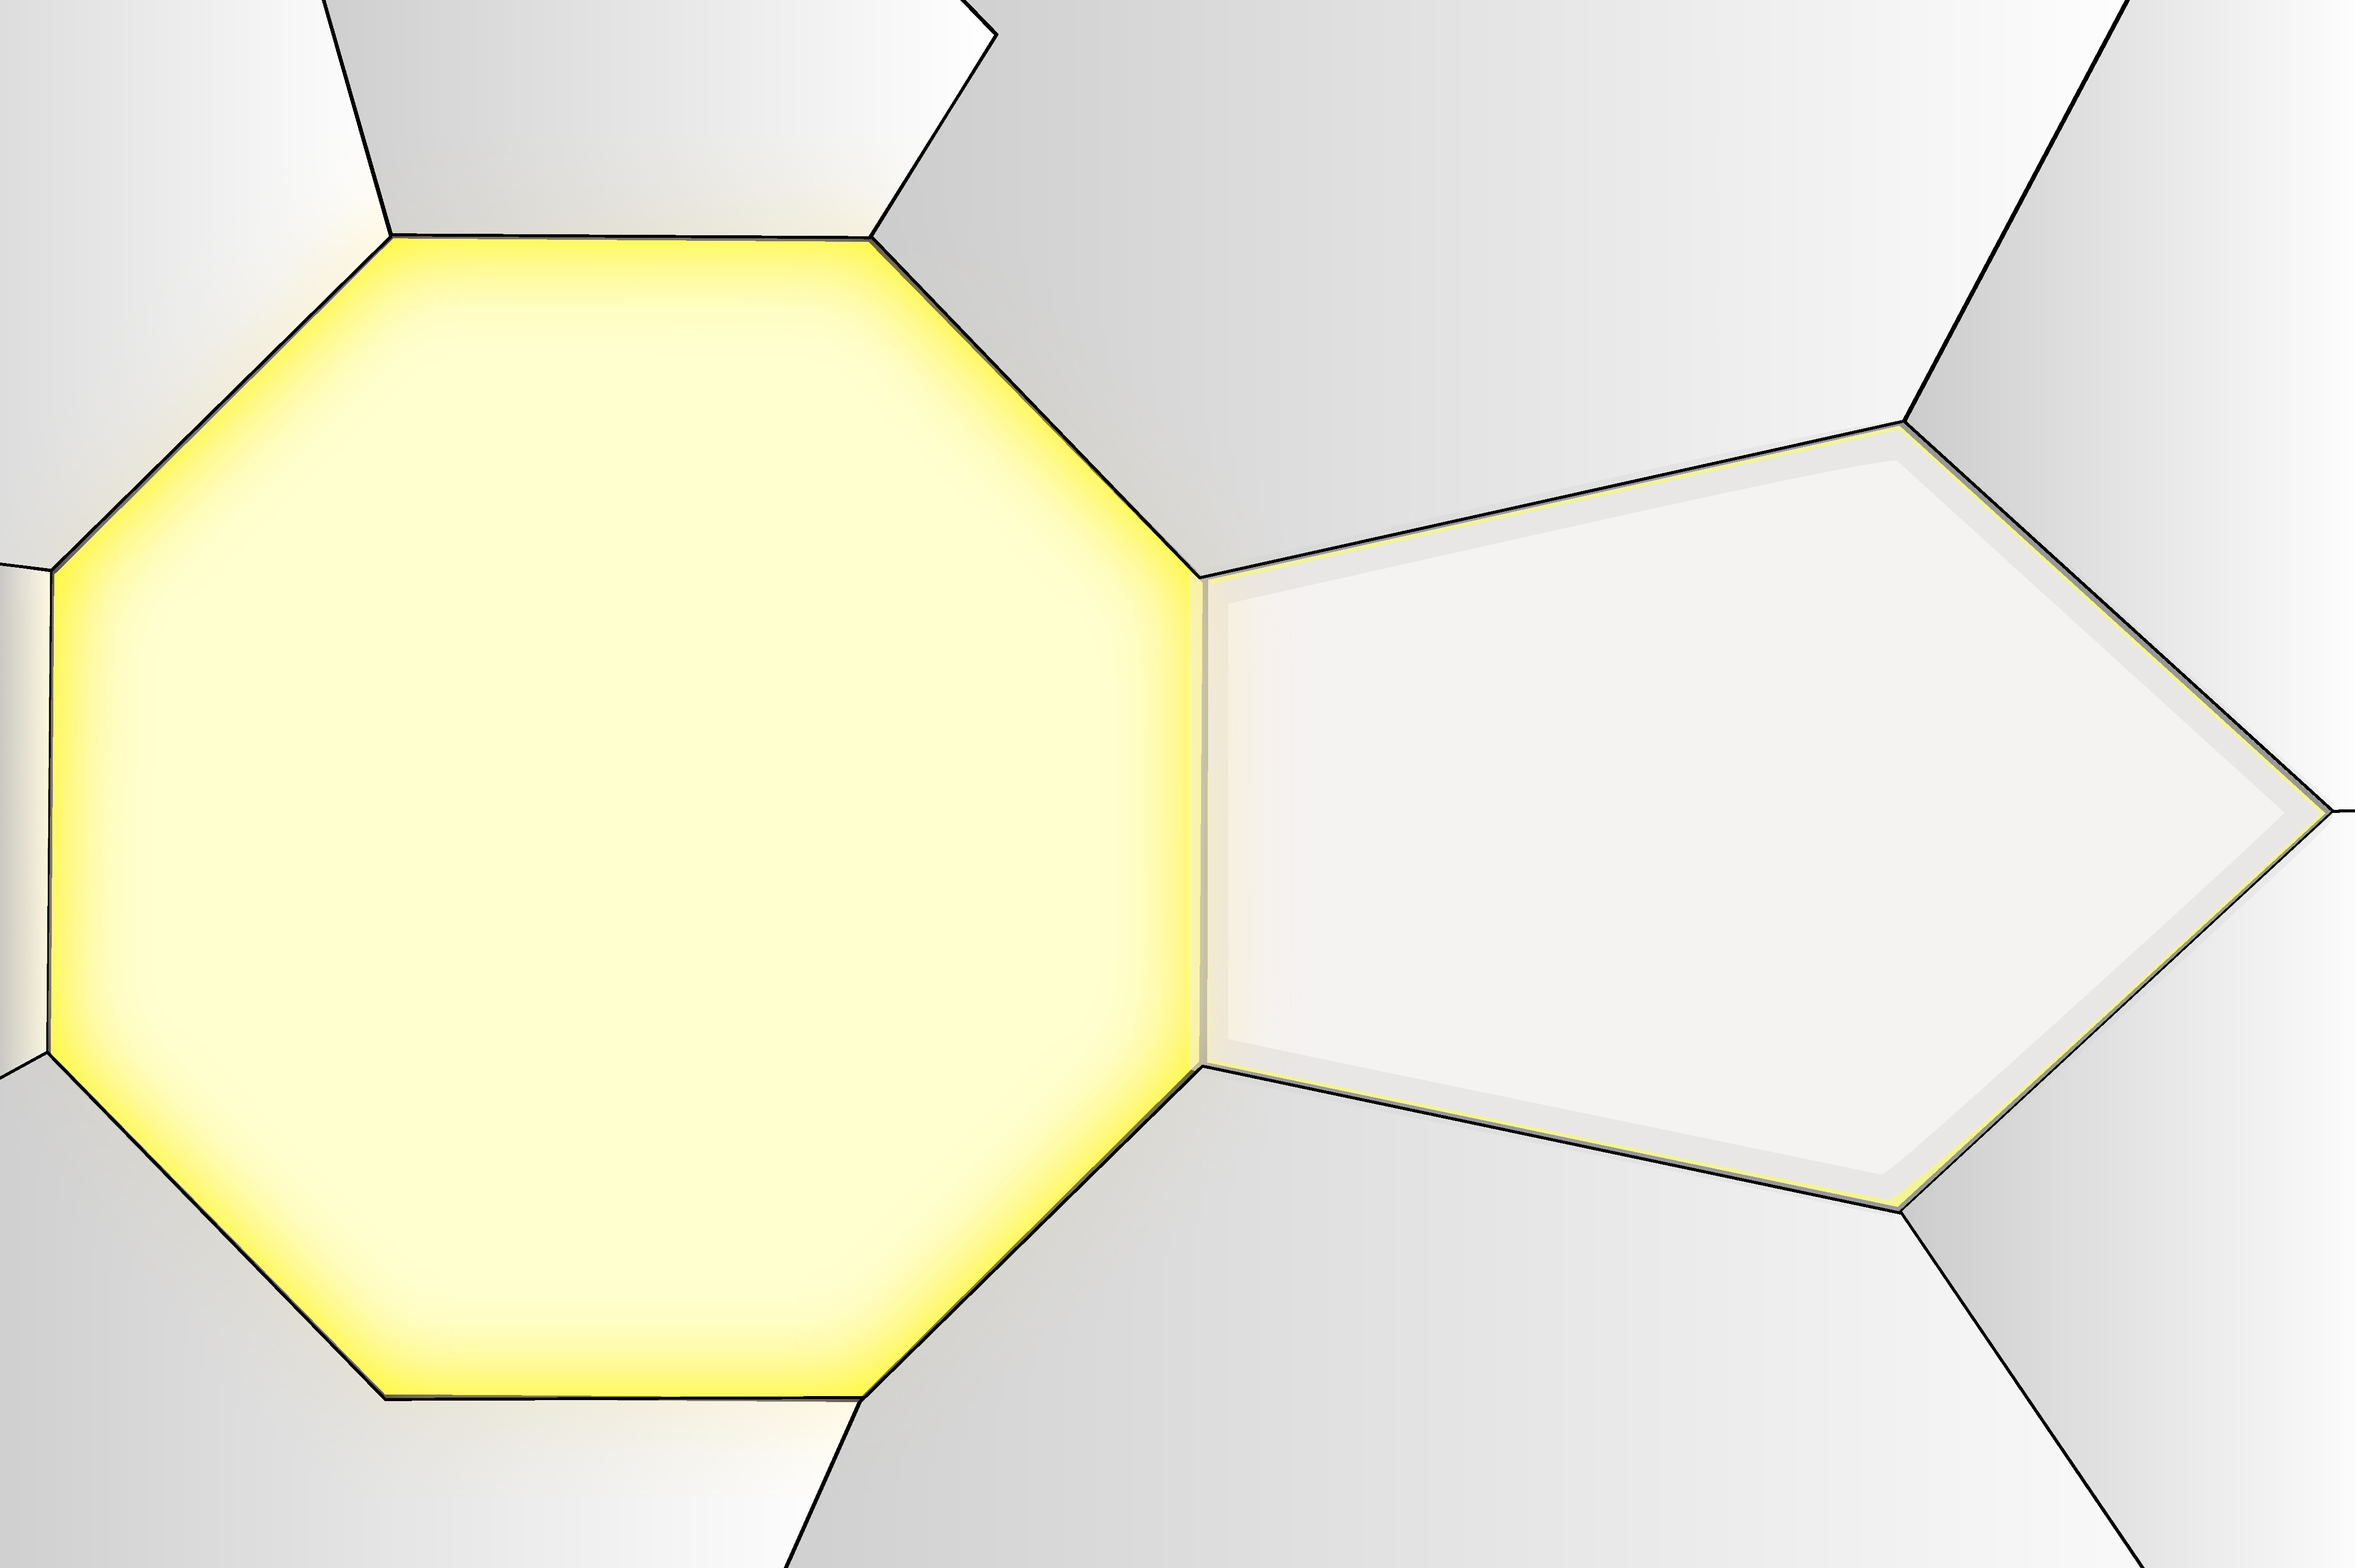
\includegraphics[width=6cm, height=4cm]{two_fes.pdf}}}
               {\frame{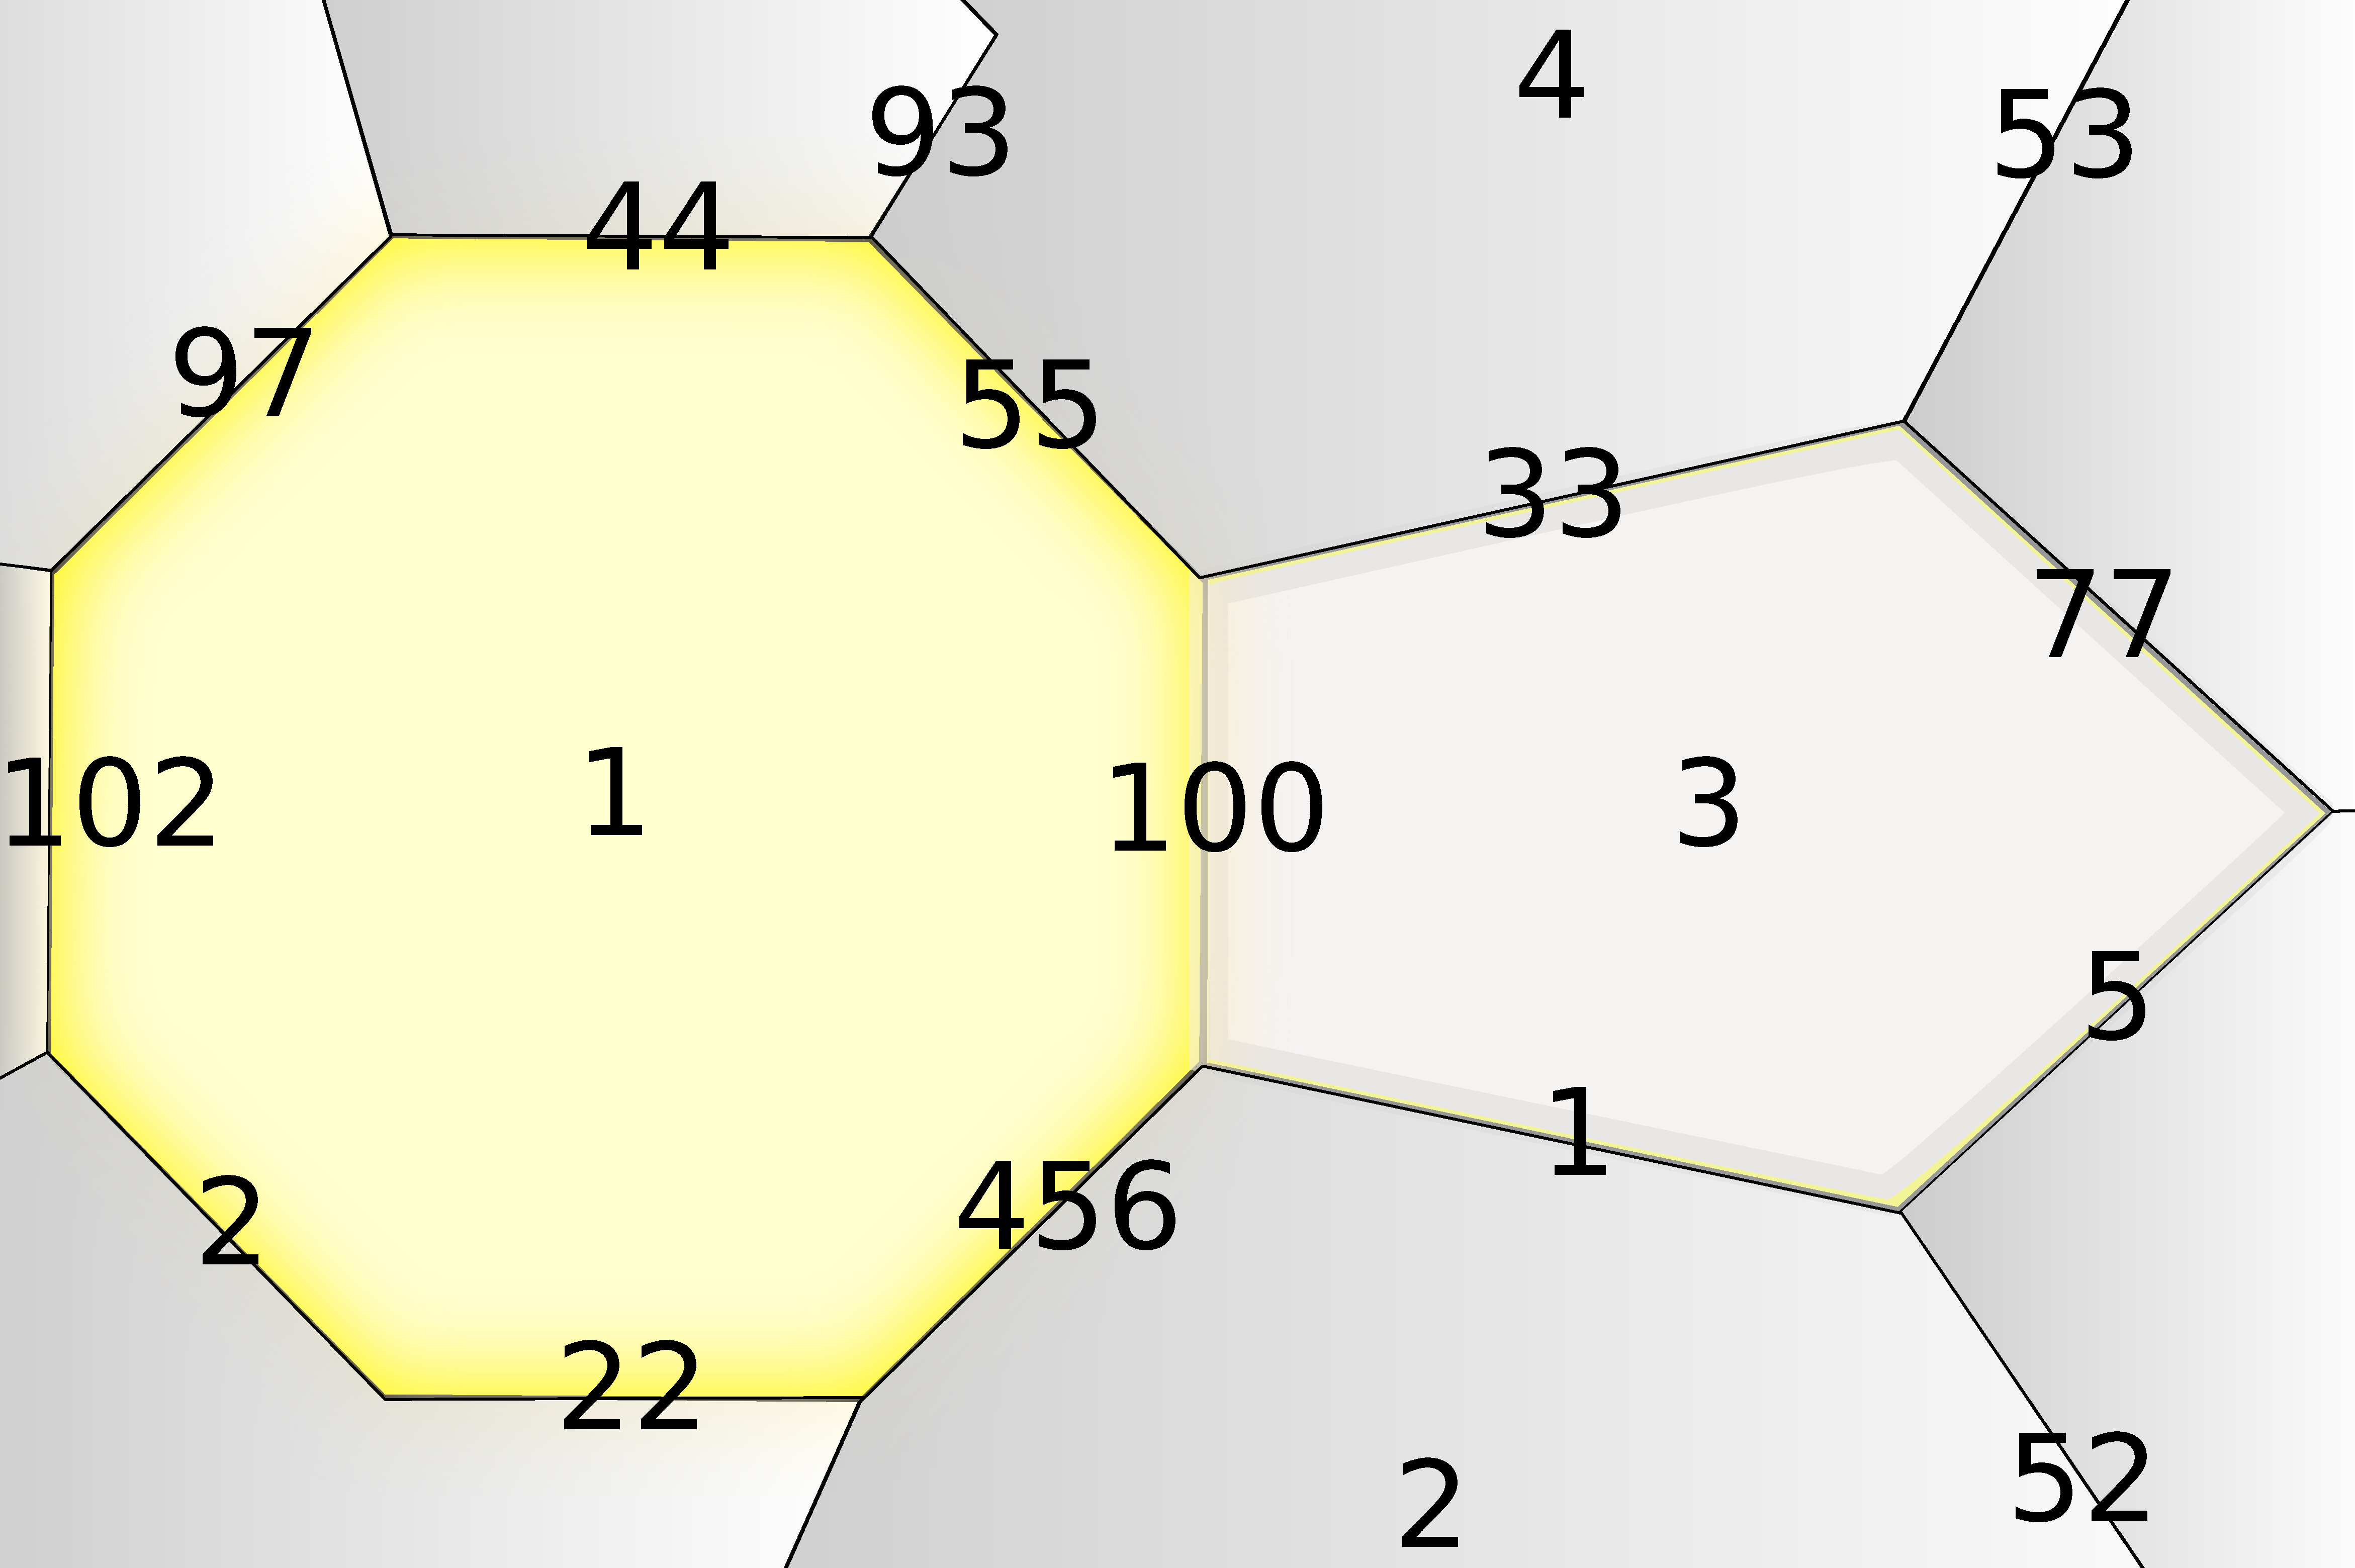
\includegraphics[width=6cm, height=4cm]{two_fes_enum_supp_faces.pdf}}}
  \end{columns}
  \begin{itemize}[<+->]
    \item Mesh will enumerate finite elements (equiv., \emph{interiors}) and non-boundary sides separately, in any order it chooses for each.
    \item Separate enumerations allow sides or fes/interiors to be dealt with separately by other components.
    \item To other components, the interior and nb side numbers are just opaque identifiers -- must ask the mesh for interpretation.
  \end{itemize}
\end{frame}
 
\subsubsection{Side Faces -- Shape Relative Side Identifiers}

\begin{frame}
  \frametitle{Side Faces -- Shape Relative Side Identifiers}
  \begin{columns}
    \column{.50\textwidth}
      \begin{itemize}[<+->]
        \item Side identifiers discussed so far are \emph{global}, and do not tell the \emph{\textbf{role}} that the side plays
          in the context of a \emph{\textbf{single oriented shape}}.
        \item The shape-relative side identifier is the \emph{\textbf{side face}}.
      \end{itemize}
    \column{.50\textwidth}
      \alt<-1> {\frame{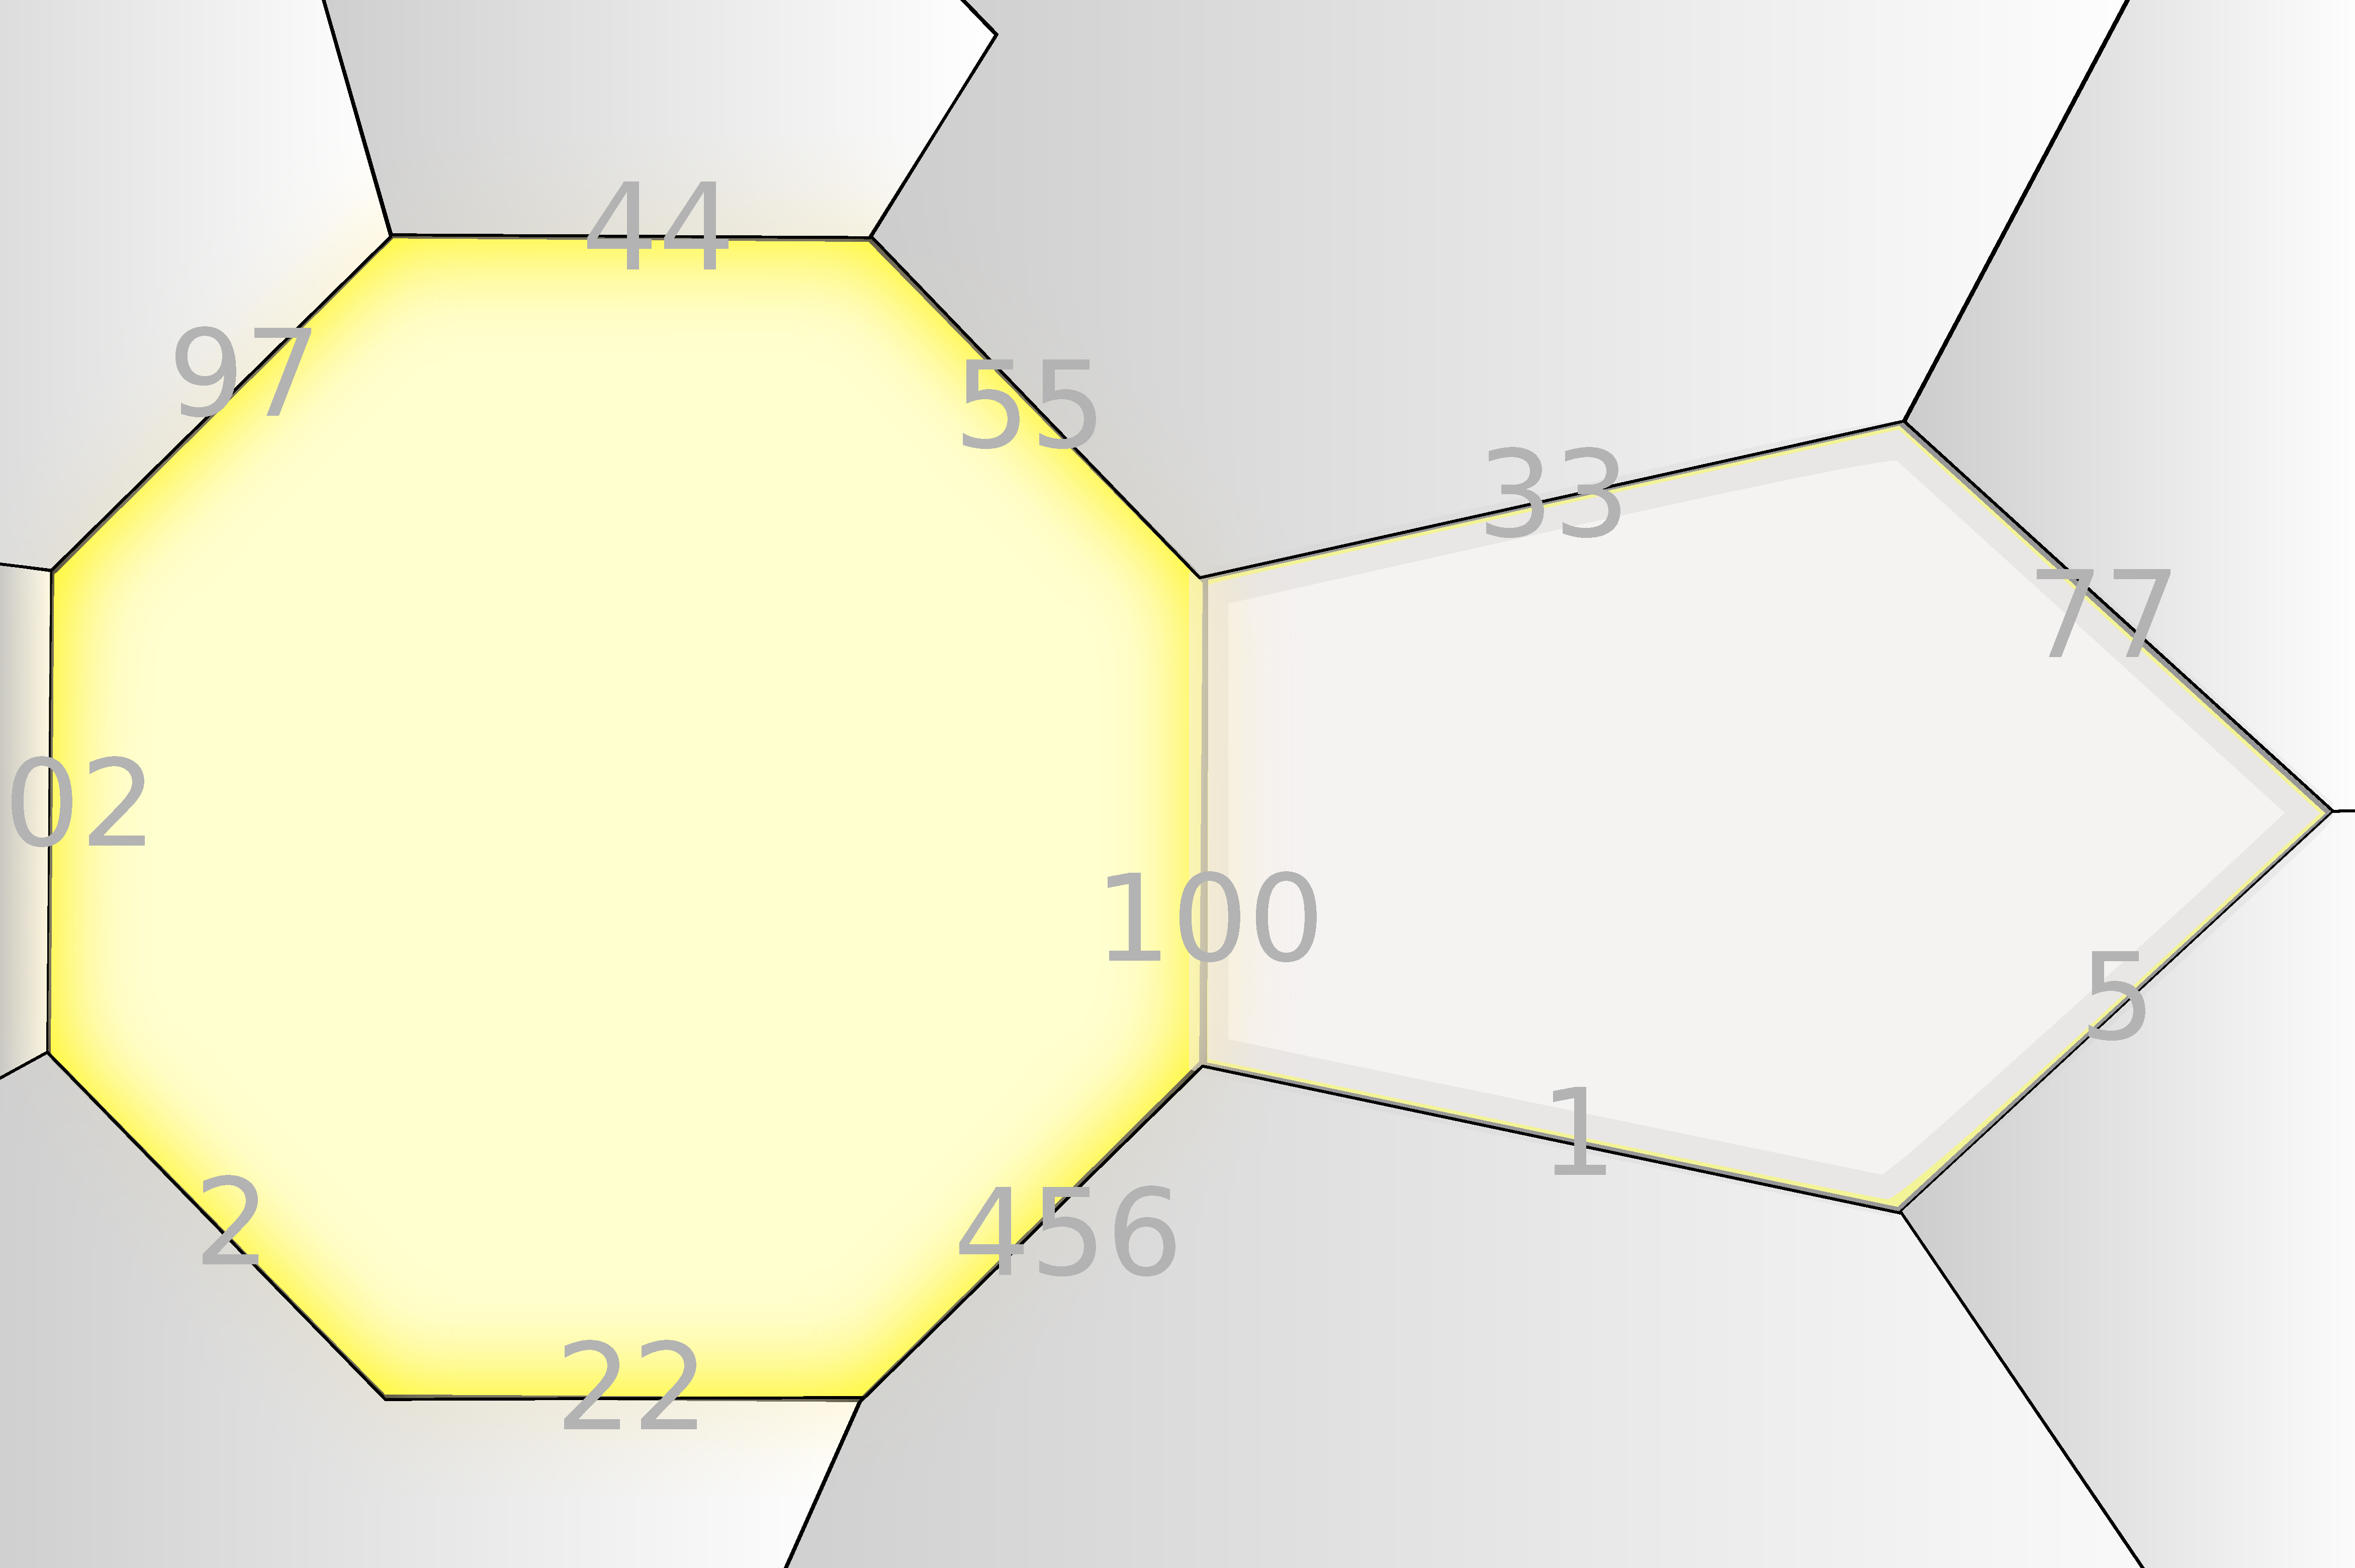
\includegraphics[width=6cm, height=4cm]{two_fes_enum_nb_side_nums_greyed.pdf}}}
               {\frame{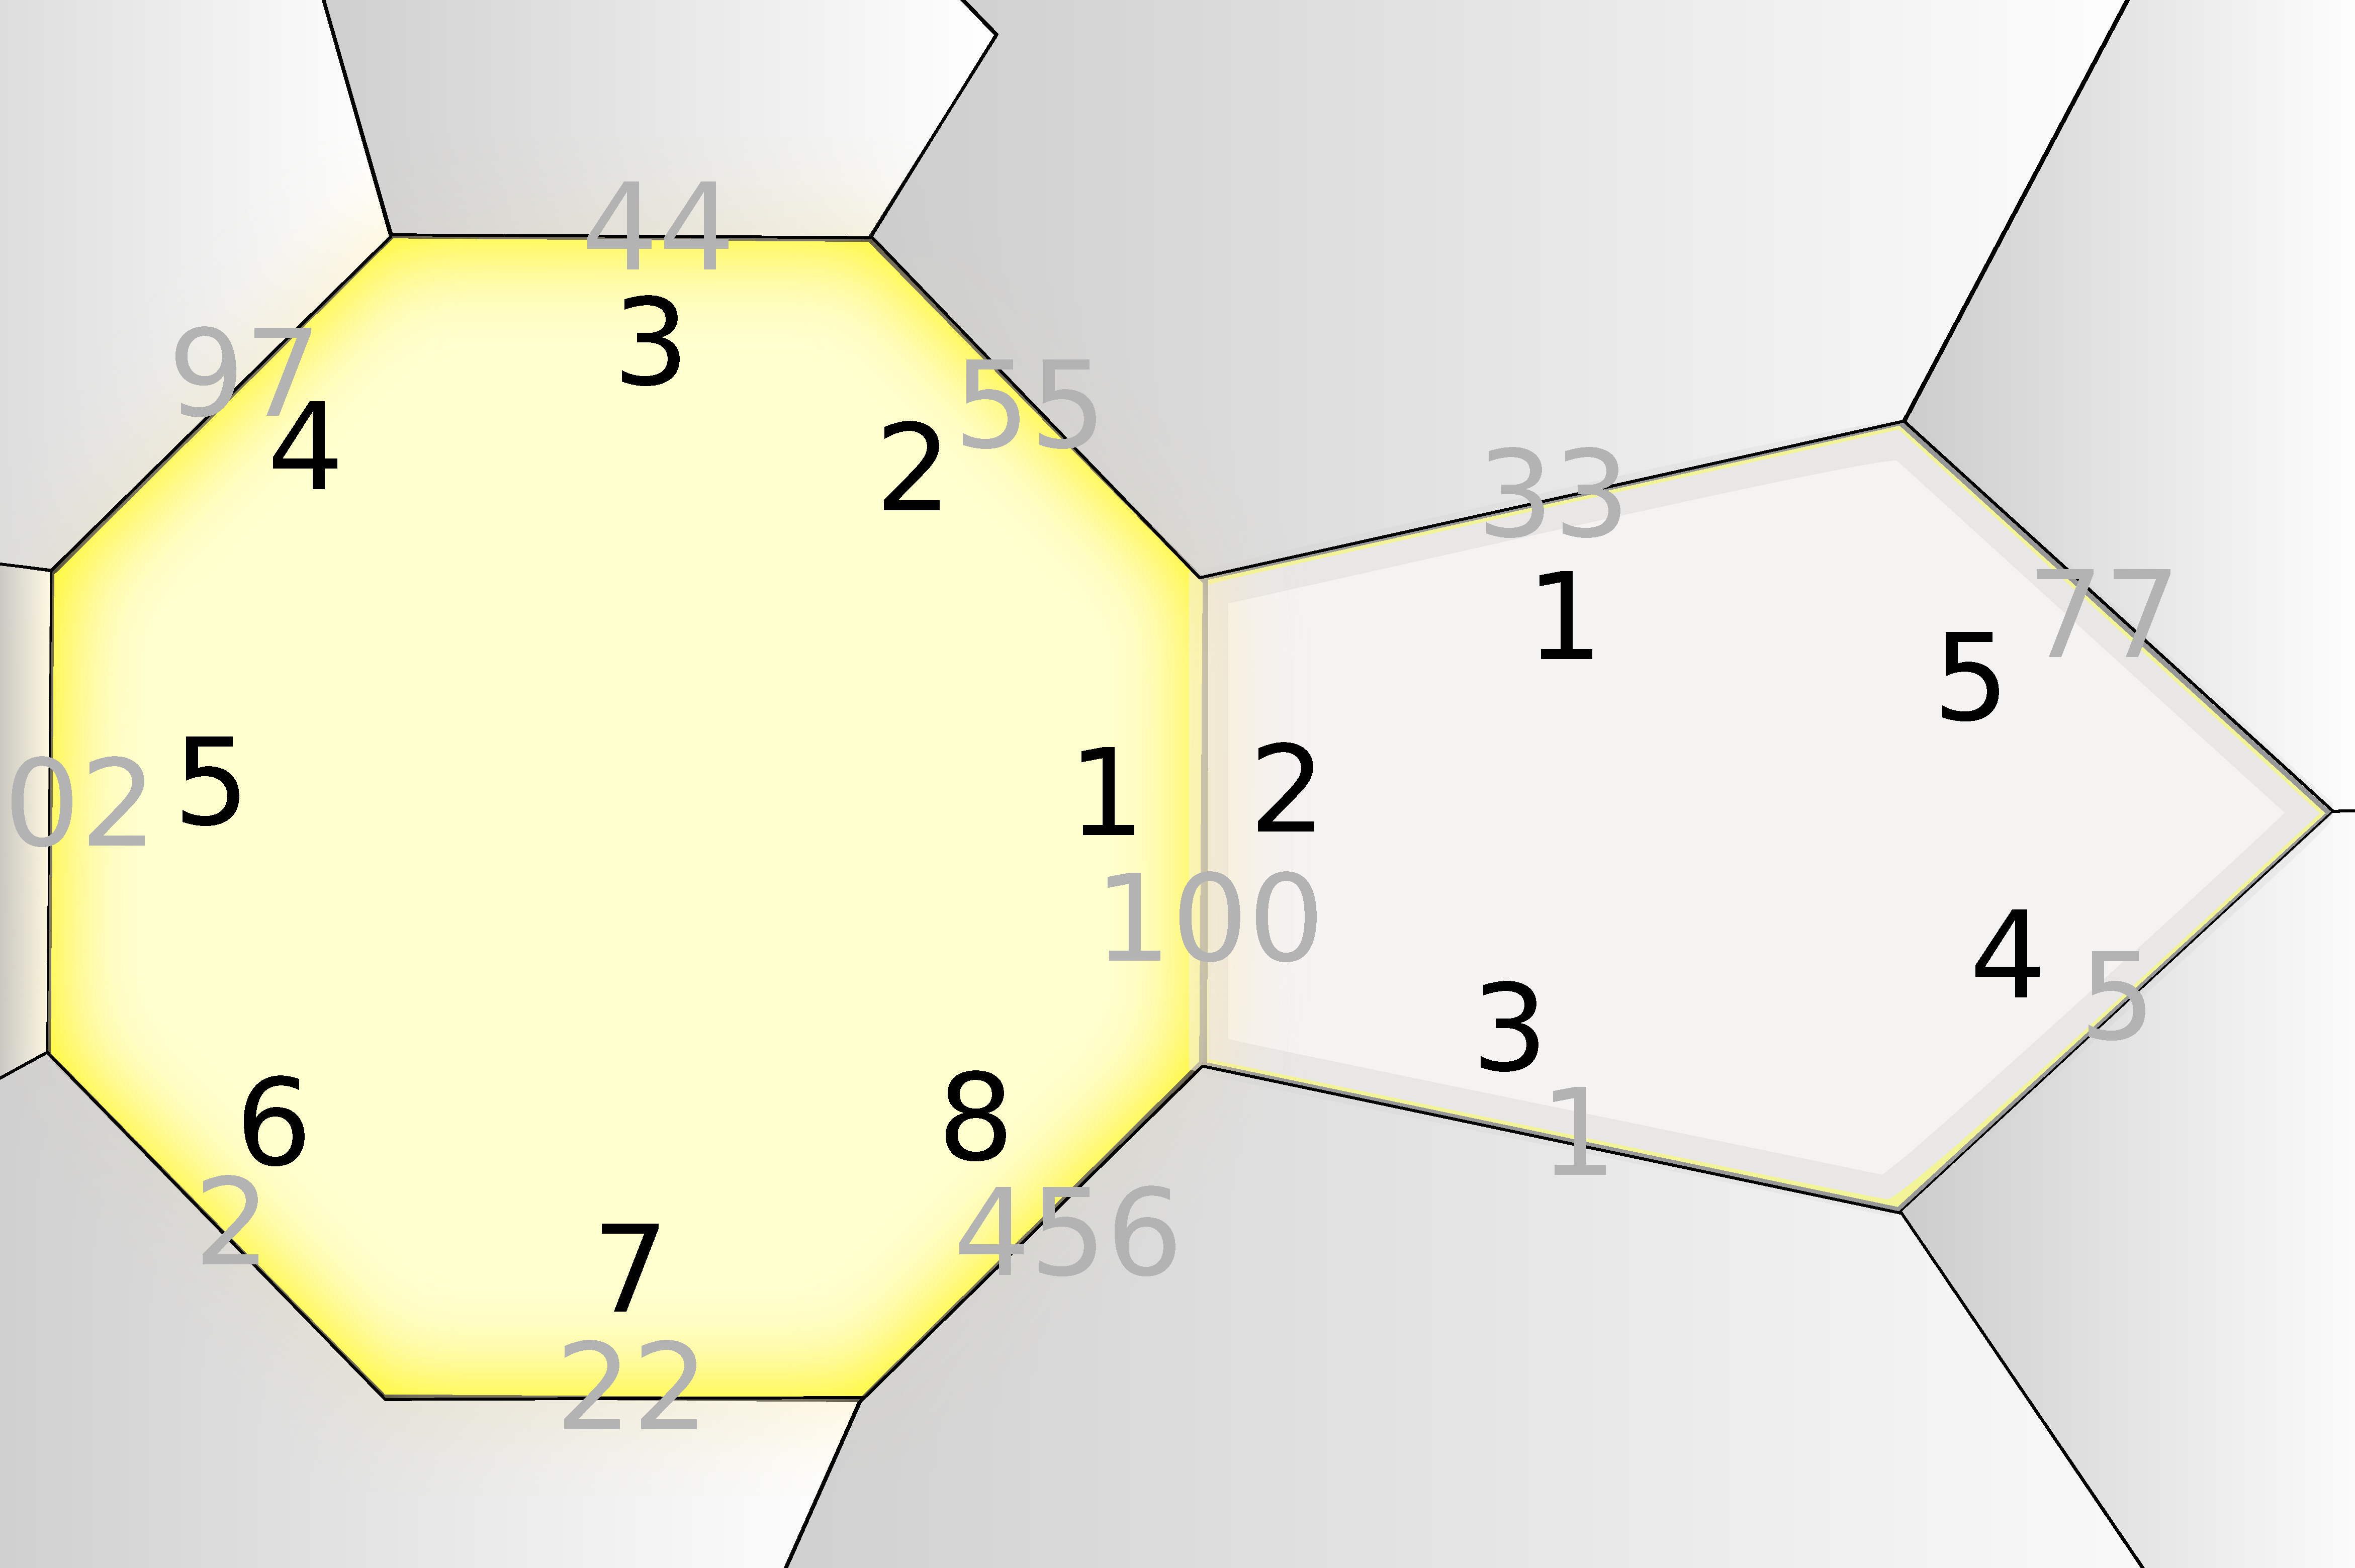
\includegraphics[width=6cm, height=4cm]{two_fes_enum_side_faces_nb_side_nums_greyed.pdf}}}
  \end{columns}
  \begin{itemize}[<+->]
    \item The sides may be numbered in any order by the mesh, each oriented shape having its own numbering.
    \item A finite element inherits side face numbers from the corresponding sides of its oriented shape.
    \item The side faces are necessary to represent sides in computations involving geometry (e.g. integrals)
      on oriented shapes and finite elements.
  \end{itemize}
\end{frame}
 
\subsubsection{FE/Side Faces Including a Non-Boundary Side}

\begin{frame}
  \frametitle{FE/Side Faces Including a Non-Boundary Side}
  \begin{columns}
    \column{.50\textwidth}
      \begin{itemize}[<+->]
        \item Mesh will need to provide identifiers for the \emph{\textbf{support faces}} for the basis shape functions.
        \item Only interiors and non-boundary sides will host shape functions.
      \end{itemize}
    \column{.50\textwidth}
      \alt<-2> {\frame{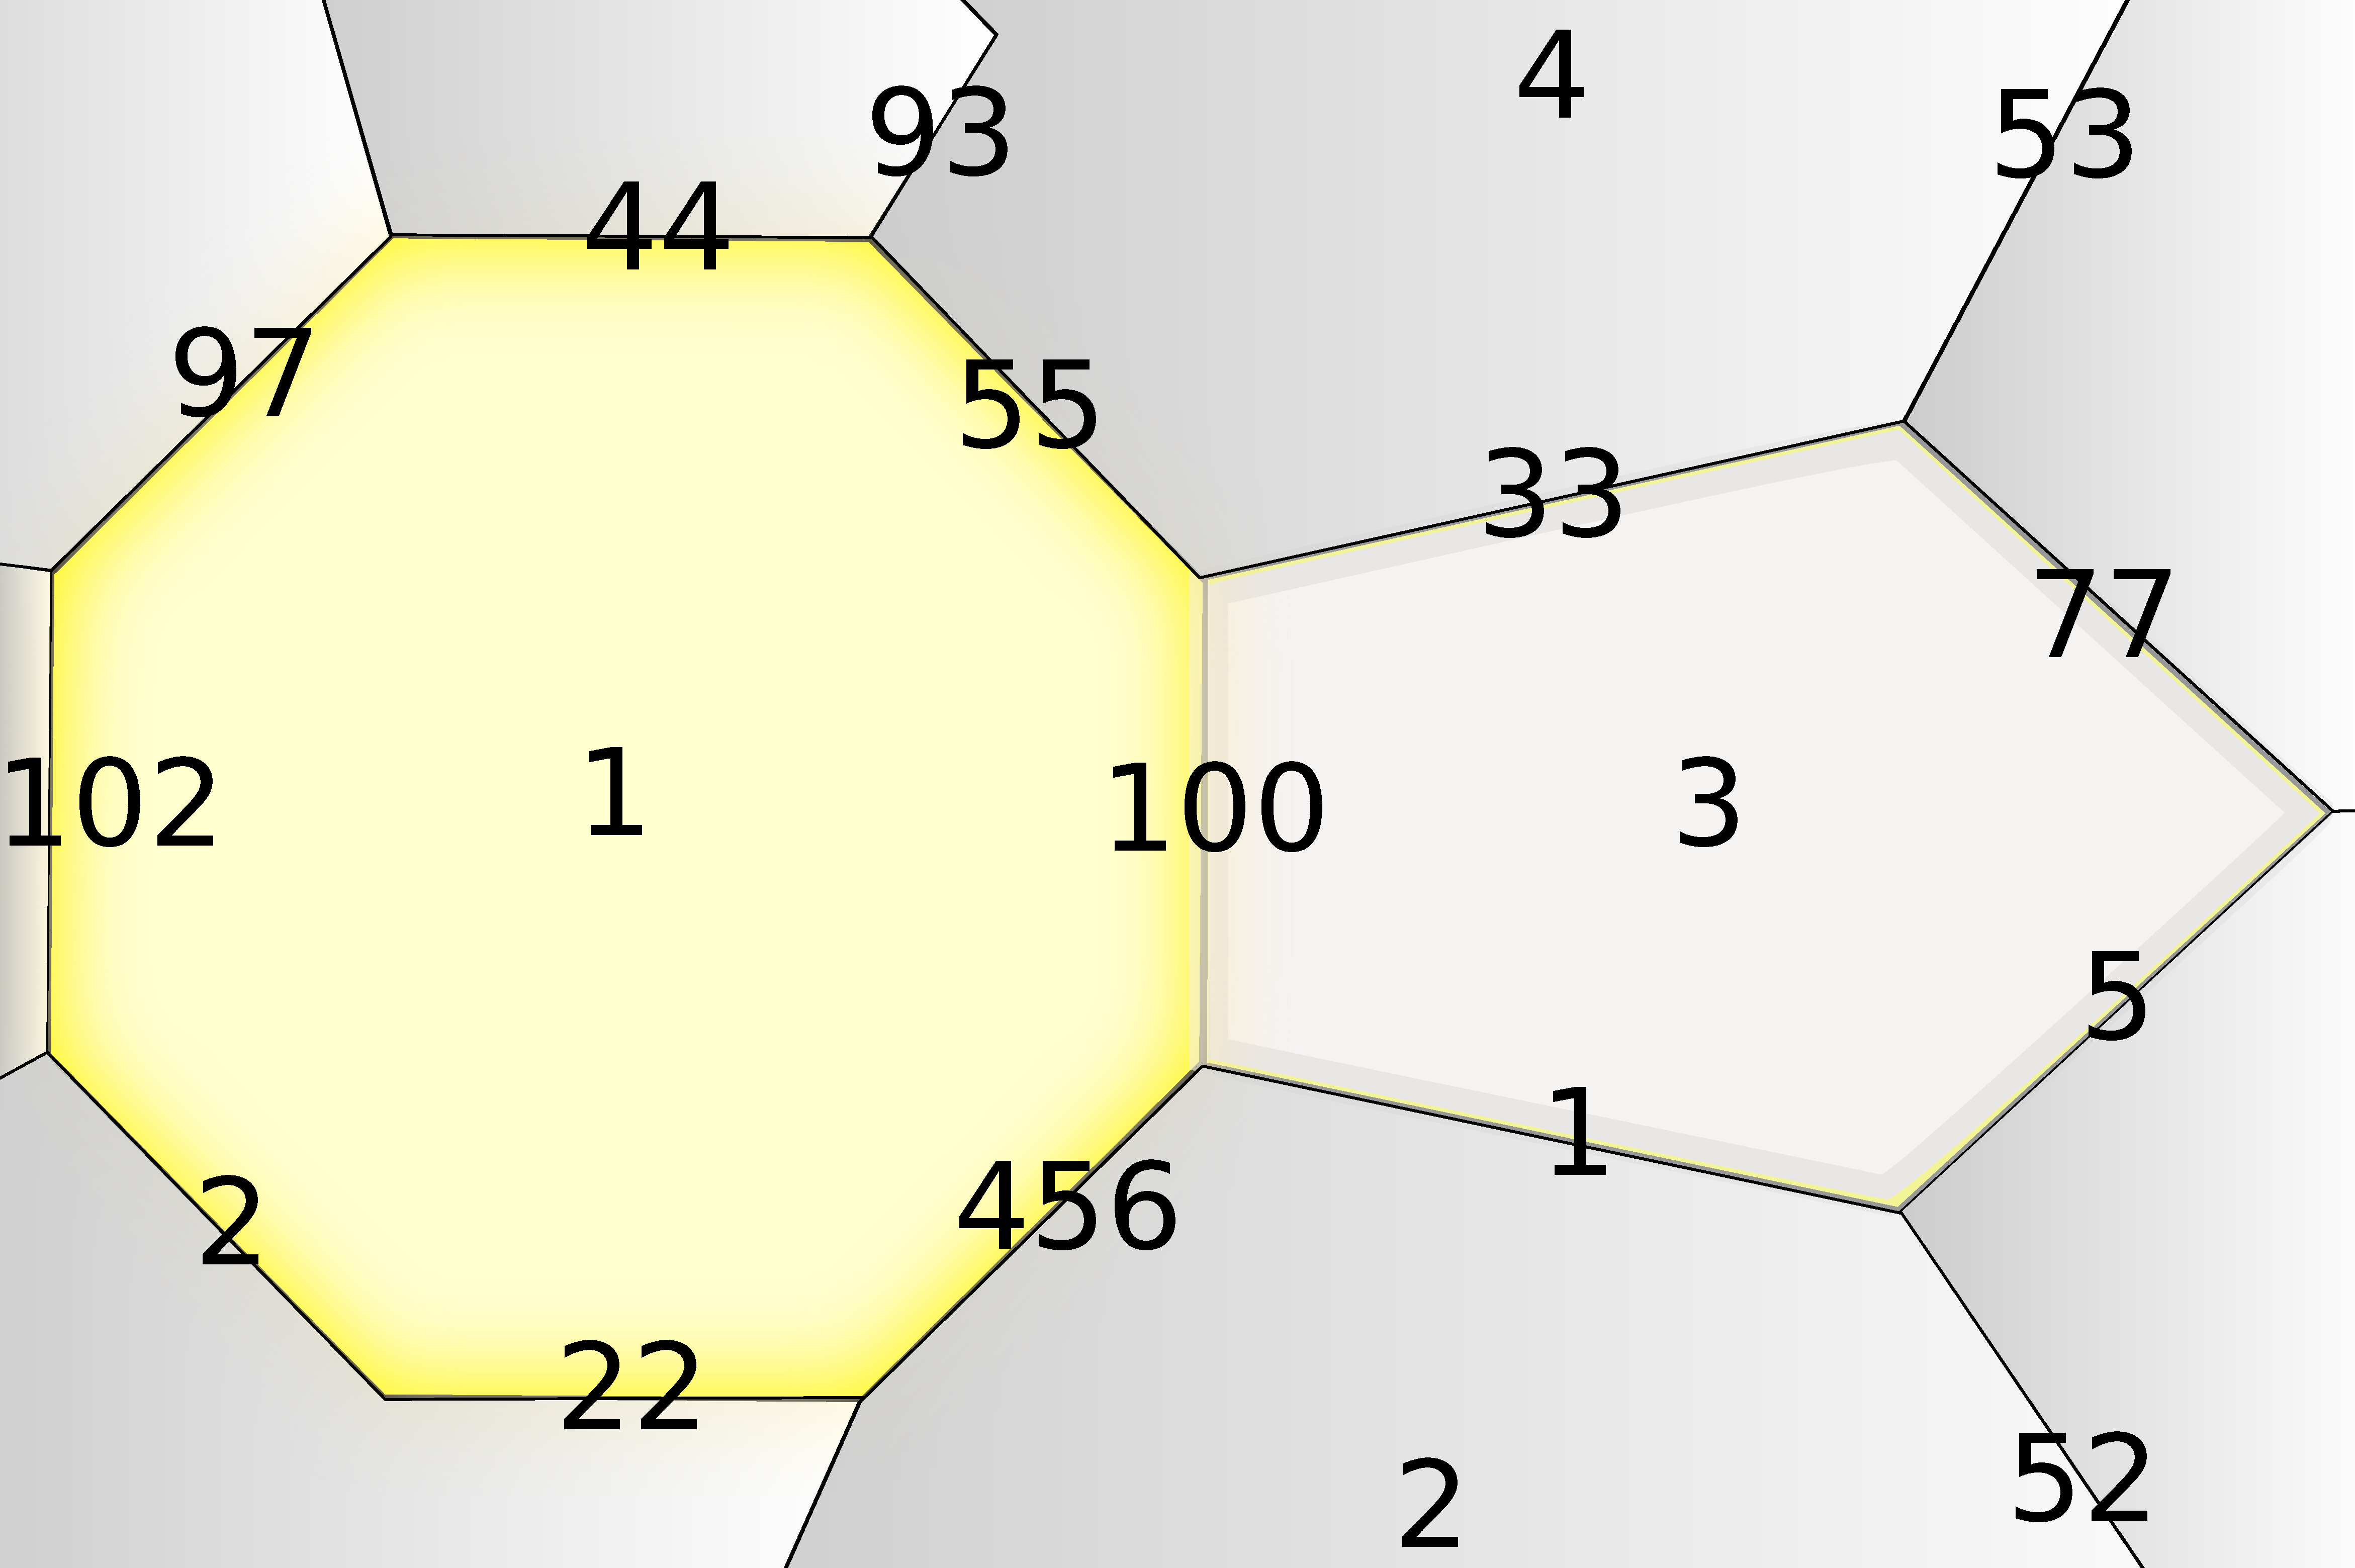
\includegraphics[width=6cm, height=4cm]{two_fes_enum_supp_faces.pdf}}}
               {\frame{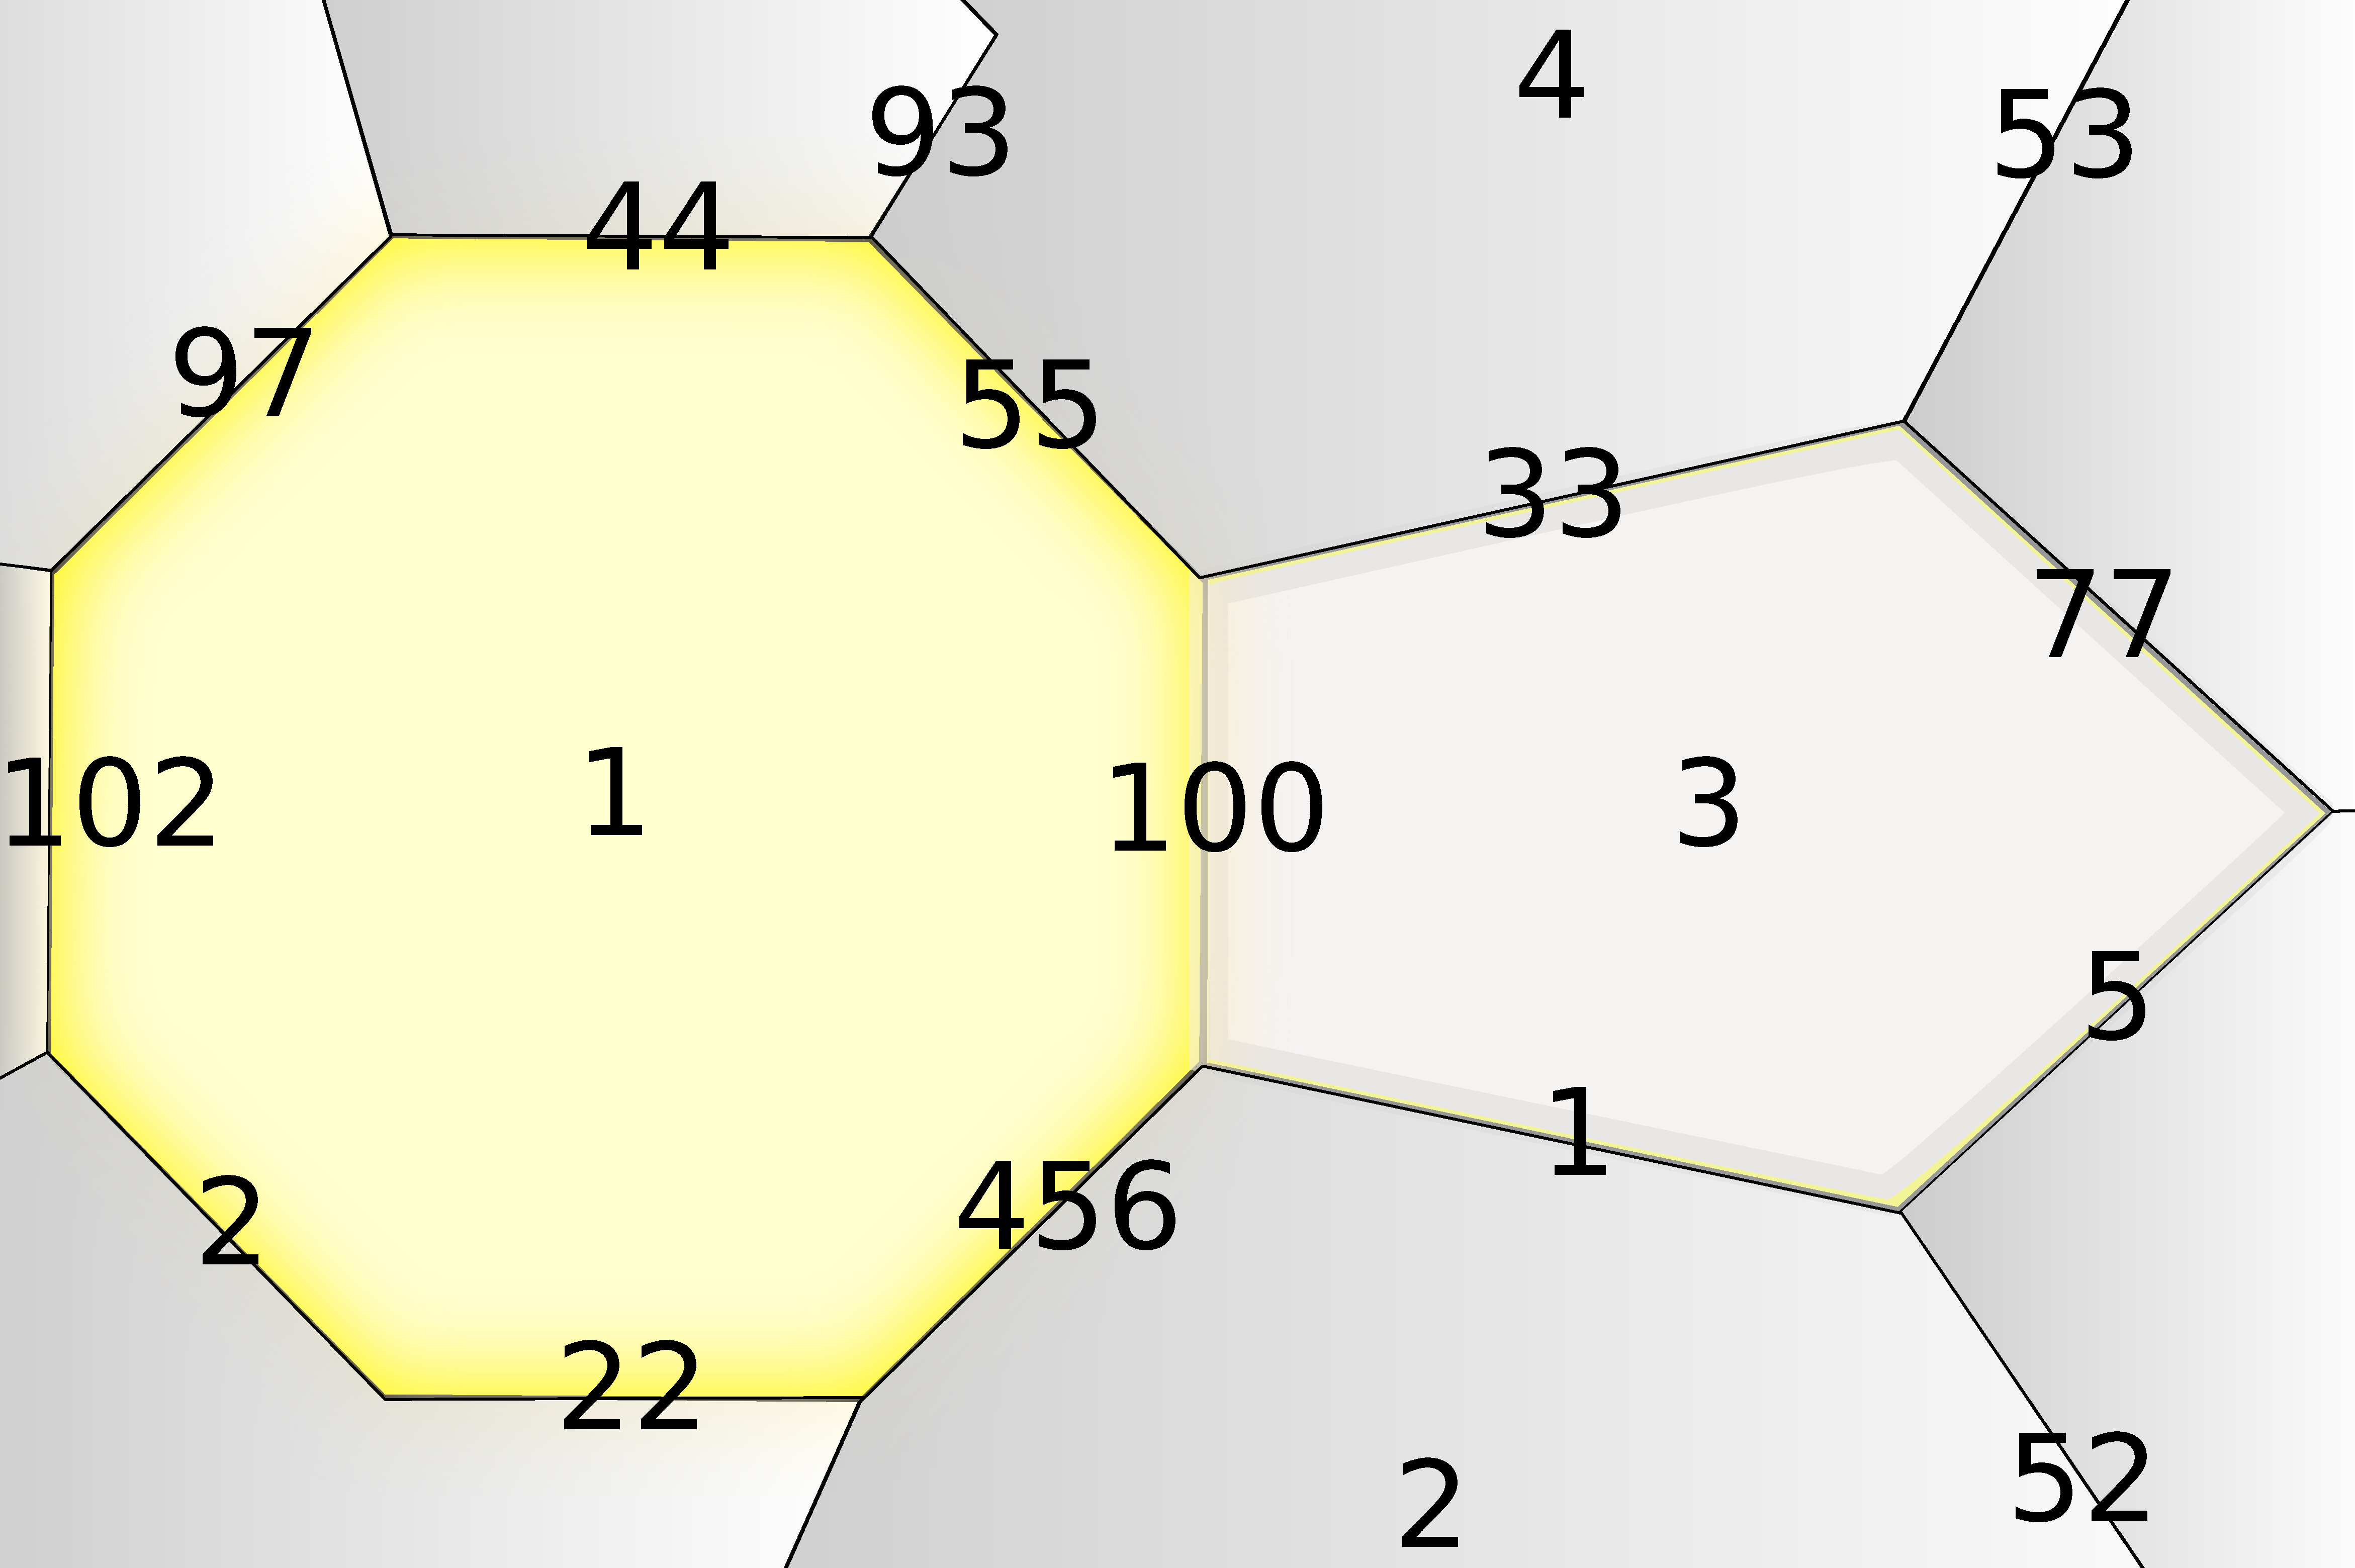
\includegraphics[width=6cm, height=4cm]{two_fes_enum_supp_faces.pdf}}}
  \end{columns}
  \begin{itemize}[<+->]
    \item Mesh will enumerate finite elements (equiv., \emph{interiors}) and non-boundary sides separately, in any order it chooses for each.
    \item Separate enumerations allow sides or fes/interiors to be dealt with separately by other components.
    \item To other components, the interior and nb side numbers are just opaque identifiers -- must ask the mesh for interpretation.
  \end{itemize}
\end{frame}


%We'll require of our meshes that any non-boundary side is included (ie is a subset of) in exactly two finite elments,
%and has no significant intersection with any other (the intersection has no measure in d-1 dimensional space).

%Too Restrictive?  What About Hanging Nodes?
%(Add diagram: of hanging node) If we need more refinement on one side than the other, leaving hanging nodes, we'll just define each piece
%to be a side (which meet at a straight angle), so these cases are easily handled with this assumption.

%Now we are able to introduce the idea of the Non-Boundary Side Inclusions (or "Inclusions" for short) of a non-boundary side.
%Def: The Non-Boundary Side Inclusions of a given non-boundary side are the pair of (fe, side-face) pairs of the two finite elements
     %which include the side.
  %(Structure)
    %fe1
    %side_face_in_fe1
    %fe2 identifier
    %side_face_in_fe2
%Note use of fe-local side-face identifiers.


\end{document}

